\documentclass[DM,authoryear,toc]{lsstdoc}
% lsstdoc documentation: https://lsst-texmf.lsst.io/lsstdoc.html
\input{meta}

% Package imports go here.
\usepackage{graphicx}
\usepackage{hyperref}

% Local commands go here.

\title{AWS Proof of Concept Project Report}

\author{
Hsin-Fang Chiang,
}

\setDocRef{DMTN-137}
\setDocUpstreamLocation{\url{https://github.com/lsst-dm/dmtn-137}}

\date{\vcsDate}

\setDocAbstract{%
From April to December 2019, team members from LSST-DM, AWS, and HTCondor undertook a proof-of-concept project to do LSST processing on the AWS platform. This document reports the results.
}

% Change history defined here.
% Order: oldest first.
% Fields: VERSION, DATE, DESCRIPTION, OWNER NAME.
% See LPM-51 for version number policy.
\setDocChangeRecord{%
  \addtohist{1}{YYYY-MM-DD}{Unreleased.}{Hsin-Fang Chiang}
}


\begin{document}

% Create the title page.
%\maketitle
% Frequently for a technote we do not want a title page  uncomment this to remove the title page and changelog.
% use \mkshorttitle to remove the extra pages
\mkshorttitle

\newcommand{\poc}{AWS PoC}

\lstdefinestyle{basherror}{
  language=bash,
  showspaces=false,
  showstringspaces=false,
  breaklines=true,
  postbreak=\mbox{\textcolor{red}{$\hookrightarrow$}\space},
  basicstyle= \tiny \ttfamily
}


\lstdefinestyle{sqlprompt}{
  language=SQL,
  showspaces=false,
  showstringspaces=false,
  breaklines=true,
  postbreak=\mbox{\textcolor{red}{$\hookrightarrow$}\space},
  numbers=left,
  numberstyle=\tiny,
  commentstyle=\color{gray},
  basicstyle=\tiny \ttfamily,
}


\section{Background}

In April 2019, LSST Data Management (DM) began a proof of concept (PoC) project with the Amazon Web Services (AWS) and HTCondor teams to explore whether a cloud deployment of the LSST Data Release Production (DRP) is feasible.
The execution plan is in \citeds{DMTN-114}.
For this project AWS granted us credits to use their platform.
The team met biweekly to discuss progress and plans.

In this document we report on the work carried out, results obtained, and lessons learned with respect to the technologies used, the LSST code base, and the overall PoC process.
We first list the relevant technologies in Sect \ref{sec:tech}, and Sect \ref{sec:arch} describes how they were used to execute the DRP workflow.
In Sect \ref{sec:approach} we discuss certain principles that were helpful in ensuring progress and success.
The modifications to the Data Butler that were necessary to execute in the cloud environment are detailed in Sect \ref{sec:butler}.
Results of scaling tests and cost estimates are given in Sect \ref{sec:results}.
Finally, potential improvements or extensions and lessons learned are listed in Sect \ref{sec:future}.

\section{Technology stack} \label{sec:tech}

\subsection{Amazon Elastic Compute Cloud (EC2)}

\href{https://aws.amazon.com/ec2/}{Amazon Elastic Compute Cloud (EC2)} service provides secure, resizable compute capacity in the cloud based on virtualization technologies.
The unit of compute resources is an instance, and users can scale up and down the number of instances.
EC2 instances come with multiple instance types for a configuration of memory, CPU, and storage.
An Amazon Machine Image (AMI) bundles the Operating System (OS) with required data and configurations into a convenient image that can be launched on any EC2 instance type.
\href{https://aws.amazon.com/efs/}{Amazon Elastic File System (Amazon EFS)} provides a POSIX-compliant, scalable, elastic NFS file system designed to provide parallel shared access to thousands of AWS compute instances.
We have used On-demand and Spot instances in the \poc.
On demand instances cost more but they can not be deallocated by AWS.
Spot instances are significantly cheaper, but at any time AWS, given a 2 minute warning, can request the compute resources back and deallocate them.
\subsection{Amazon Simple Storage Service (S3)}
\href{https://aws.amazon.com/s3/}{Simple Storage Service (S3)} is an object storage that allows massive amounts of unstructured data where each object typically includes data and related metadata and is identified by a globally unique identifier, to be stored and accessed from EC2 instances or elsewhere in a durable and highly scalable way.
Buckets, organizational units in which related objects are generally stored, enable easier access and privilege administration.
Access, read, write, delete and other atomic units of action on the objects themselves can be allowed or forbidden at the account, bucket or individual object level.
Logging is available for all actions on the Bucket level and/or at the individual object granularity.
It is also possible to define and issue complex conditions on Bucket or object actions which can execute arbitrary actions or workflows, but S3 itself is not POSIX compliant.
\subsection{PostgreSQL}
PostgreSQL is one of the most popular open source relational database systems available.
\href{https://aws.amazon.com/rds/}{Relational Database Service (RDS)} is the AWS cloud service that launches and configures databases with ease.
The RDS databases can be backed up into snapshots as well as exported to downloadable files on S3.
Besides no additional licensing fees usually associated with proprietary software, PostgreSQL's off-the-shelf support for spatial primitives needed for astronomy was the primary reason of choosing it.
While LSST (via Qserv) has demonstrated similar primitives on MariaDB, the ease of deploying PostgreSQL in RDS, the common use of PostgreSQL as a Virtual Observatory (VO) Table Access Protocol (TAP) backend, and the desire to demonstrate portability of the Butler code were desirable factors.
\subsection{HTCondor}
\href{https://research.cs.wisc.edu/htcondor}{HTCondor}\citep{condor-practice} provides distributed job parallelization and is a powerful batch system for high throughput computing (HTC).
A HTCondor pool is a collection of compute resources, and HTCondor matches job requests with available resources following their job requirements.
HTCondor Annex allows HTCondor deployment on cloud resources via acquisition of cloud compute resources external to an existing HTCondor pool.
A HTCondor pool can have multiple annexes, and each annex manages its own lifecycle.
Instances allocated by \texttt{condor\_annex} are added to a shared resource pool on which jobs can be scheduled.
Unused compute resources are automatically deallocated after some set time spent idling.
HTCondor has been succesfully used by \href{https://aws.amazon.com/blogs/aws/experiment-that-discovered-the-higgs-boson-uses-aws-to-probe-nature}{the HEP Cloud project}, scaling up to 60,000 cores in a multi-region deployment on AWS, and by \href{https://www.linkedin.com/pulse/using-50k-gpus-across-multiple-clouds-icecube-science-igor-sfiligoi}{the IceCube experiment}, where they scaled up to 51,000 GPUs across multiple regions and multiple cloud providers (AWS, Azure, and Google Cloud).
\subsection{Pegasus}
\href{https://pegasus.isi.edu/}{Pegasus}\citep{deelman-fgcs-2015} is a workflow management system built on top of HTCondor.
Popular in large-scale scientific computing, it provides command line and API interfaces for scientists to write an abstract workflow independent of the underlying computing infrastructure.
Pegasus workflows are expressed as Directed Acyclic Graphs (DAGs) where jobs are the nodes and job dependencies are represented by the edges.
Pegasus utilizes HTCondor DAGMan as its execution engine, but also supports various execution environments and data management strategies.
\subsection{LSST Software Stack}
The \href{https://pipelines.lsst.io/}{LSST Science Pipelines Software Stack} is a collection of data processing codes for optical and near-infrared astronomy, and is used for DRP \citep{2018PASJ...70S...5B}.
Besides image processing and astronomical catalog analysis, it includes a middleware layer for data access, task definition and execution.
The LSST Data Butler is a framework that abstracts the underlying data persistence and implementations from Science Pipelines algorithms, and a data repository is a set of datasets under control of the Data Butler \citep{2018arXiv181208085J}.
The Data Butler concepts can be found in \citeds{LDM-463}.
"The middleware layer is in the course of a major redesign and refactoring, the new version is known as the Generation 3 Middleware ("Gen3" Middleware; \citeds{DMTN-056}).
This \poc~added new features in the Generation 3 Data Butler; see Sect \ref{sec:butler}.


\section{Architecture design} \label{sec:arch}


The system at the end of the PoC is shown in Figure~\ref{fig:arch}.
All components are hosted on the AWS platform.

\begin{figure}
  \centering
  \includegraphics[width=\textwidth]{figures/arch}
  \label{fig:arch}
  \caption{Diagram of the AWS PoC system architecture.}
\end{figure}

AMIs containing the LSST Software Stack, Pegasus, and a configured HTCondor installation are pre-built in two flavors: master and worker.
These contain the complete environment required to run DRP workflows and scale them out with HTCondor.
The user launches an on-demand EC2 instance using the master AMI to be the submit host and the central manager of the HTCondor pool.
The user logs in to this master to control the workflow execution.

The LSST DRP workflow in the Generation 3 Middleware is represented as a Directed Acyclic Graph (DAG) known as a Quantum Graph.
In the Generation 3 Middleware, a Pipeline Task represents a configured sequence of a data processing operation, and defines the inputs and outputs used in conjunction with the Data Butler.
Each executable unit, known as a Quantum, represents a single execution of a particular Pipeline Task with particular inputs producing particular outputs.
The Quantum Graph is aware of the Quantum dependency and determines the execution workflow.
For simplicity we map each Quantum to a standalone job, although this may not be optimal for performance (grouping multiple Quanta into a single job can reduce or amortize overhead).
Pegasus is used to submit the workflow to HTCondor as well as monitor the workflow execution.
Pegasus adds other necessary jobs, such as data transfer, to the executable workflow.
HTCondor DAGMan is the workflow execution engine behind Pegasus and controls the processes.

Compute resources are procured from the master node via \texttt{condor\_annex} by targeting the worker AMI.
\texttt{condor\_annex} can request on-demand or spot instance fleets.

LSST Pipeline jobs are executed on the worker instances; they use the Data Butler for data access.
New Data Butler backends were implemented during the PoC, see Sect \ref{sec:butler}.

The Butler datastore is located in an S3 Bucket and follows the same hierarchical structure that POSIX datastore does.
Consumed and produced datasets are read and written directly from S3 as bytes, whenever possible, and only downloaded to temporary files for objects whose formatters do not support serialization.
Since the directory structure is preserved by the S3 datastore the entire data repository is trivially transferable between the cloud and a local filesystem.

The Butler registry is an RDS PostgreSQL database that keeps track of all LSST science files.
Files that are not managed by Data Butler are managed by the Condor File IO via Pegasus.
These include the Data Butler configuration file, pipeline definition (Quantum) files, and the log files.
The master instance serves as the staging site for these files.
Pegasus and HTCondor manage data transfer of these files between the master and the workers; instances do not share a filesystem.


\section{Approaches and strategies} \label{sec:approach}

\poc's goal is to demonstrate that running Data Release Production (DRP) on AWS is possible.
The following approaches were taken.

\subsection{Progress in phases}

\citeds{DMTN-114} proposed development phases that broadly outlined how progress can be made and when performance would be monitored.
The outlined plan was to move the execution to AWS without any backend modifications first and then gradually switch out each component to AWS.

Before this \poc, the DRP execution relied on a shared POSIX-compliant filesystem.
In the first phase Amazon EFS was used as its replacement.
The data repository, including a POSIX datastore and a SQLite registry, was entirely located on EFS, which was mounted to each of the EC2 compute instances.

Subsequently, support for the S3 datastore eliminated the need of EFS, and the PostgreSQL RDS replaced the SQLite registry.
Also, a Personal HTCondor Pool on an single EC2 instance was used before we tested the capability to launch new EC2 instances as the HTCondor workers and execute jobs.
This approach allowed us to debug and adapt more smoothly, ensuring we always had a fallback option while integrating and testing new features and components.

\subsection{Test minimally before scaling up}

Small tasks are tested before workflows of jobs, and small workflows are tested before large workflows.
The canonical \href{https://github.com/lsst/ci\_hsc}{ci\_hsc} dataset ($\sim$8GB) and the accompanying CI workflow (156 jobs) provide a minimal HSC test dataset and a representative DRP workflow and algorithms.
This test workflow is an important step in integrating new changes.
For larger scale tests we used the \href{https://jira.lsstcorp.org/browse/DM-11345}{HSC-RC2 dataset} ($\sim$1.5TB and 27075 jobs).

\subsection{Use Generation 3 Middleware}

One of the mandates in the \poc~was to use the Generation 3 Middleware (\citeds{DMTN-056}), which has been designed to ease the DRP execution and automation compared to the previous Generation 2 Middleware.
Generation 3 Middleware design is more readily extensible to alternative backends, compared to Generation 2 Middleware.
As it was still relatively early in its implementation, findings in the \poc~were fed back to the Generation 3 Middleware team and influenced its development.

On the other hand, as during the \poc~the Generation 3 Middleware has been under active development, backwards incompatible changes occurred often, and the APIs were unstable.
Furthermore, there were no integration tests when the \poc~started, and unit test coverage was incomplete.
Hence, changes often broke functionality.
Lack of a good integration test for the code written for this \poc is still a major concern going forward.

Keeping this in mind, we decided not to always follow the bleeding edge version of the middleware, updating only when necessary, such as for important bug fixes.
We believe that the specific stack versions used should not have strong impacts on the \poc~conclusions regarding the feasibility of cloud deployment of DRP.

\subsection{Focus on end-to-end execution}

Potential optimizations and further investigations were identified throughout the PoC project but were not carried out.
Some ideas are described in Sec \ref{sec:future}.


\section{Building AWS support into the Data Butler}
\label{sec:butler}

The Data Butler is the overarching data IO abstraction through which all LSST data access is mediated \citeds{DMTN-056}.
Datasets are referred to by their unique IDs, or a set of identifying references, which are then resolved through a Registry that matches the dataset IDs, or references, to the location, file format and the Python object type of the dataset.
The system that persists, reads and potentially modifies the datasets is called the Datastore.
The Registry is almost always backed by a SQL database and the Datastore is usually backed by a shared filesystem.
A major focus of the \poc~was to implement, and investigate issues related to, an S3 backed Datastore and a PostgreSQL backed Registry.

At the time the \poc~project began, Generation 3 Data Butler implemented \texttt{PosixDatastore}, a local or shared filesystem datastore, and a SqliteRegistry.
OracleRegistry followed soon after the \poc~work began.
Initially the focus was on implementing an S3 backed datastore called S3Datastore.
The interface between AWS services and LSST Stack would be based on the official AWS SDK called boto3.
In March 2019, Dino Bektesevic visited Tim Jenness for this work and implemented the early versions of a new module in the \texttt{daf\_butler} called \texttt{s3utils}, an \texttt{S3Datastore} class, the \texttt{PosixDatastore} equivalent, and a set of appropriate unit tests that demonstrated its functionality and correctness.
The unit tests for the datastore utilize the \texttt{moto} library which mocks requests and responses sent to AWS services, so that no additional external infrastructure is required to use it.
\texttt{PostgreSqlRegistry} class was implemented partially during the visit and completed shortly after the visit.
The initial implementation showcasing the required changes to the code was submitted as a Draft Pull Request \href{https://github.com/lsst/daf_butler/pull/147}{PR-147} in \texttt{daf\_butler}.

The tentative implementation revealed issues with how the Data Butler treated Uniform Resource Identifiers, or URIs, which were, at the time, not being handled correctly, as per standards defined in \href{https://tools.ietf.org/html/rfc3986}{FC-3986}, by the \texttt{Location} class.
In May 2019 \jira{DM-19916} resolved the issues with the \texttt{ButlerURI} class.
Major efforts were then invested into refining the newly added code to the level of production quality as well as updating the remaining Generation 3 Butler to use the updated \texttt{ButlerURI} code instead.
Every call to OS functionality had to be generalized to take a URI and from it determine the appropriate operation - a call to OS functionality, a AWS operation or something else.
This led changes in \texttt{Butler}, \texttt{Config}, \texttt{ButlerConfig} and YAML Loader classes.
These changes made the design of Data Butler more general and readily extesible to alternative cloud providers.

Further integration of the S3 backend required a change to Formatter classes to enable data serialization and deserialization to and from bytes.
Formatters present interfaces for reading and writing of Python objects to and from files.
They are the mechanism underlying how Data Butler is capable of presenting data as science products in the form of Python objects, abstracting away the underlying file types.
Modifications were made to \texttt{JsonFormatter}, \texttt{PickeFormatter}, \texttt{YamlFormatter}, \texttt{PexConfigFormatter} and the generic abstract class \texttt{Formatter}.
This concluded the last of changes required for \texttt{S3Datastore} integration and the code was merged in \href{https://github.com/lsst/daf_butler/pull/179}{PR-179} in \texttt{daf\_butler} (\jira{DM-13361}).
It became apparent that similarities were shared between \texttt{PosixDatastore} and \texttt{S3Datastore}, and would be shared by other future datastore implentations.
This prompted \jira{DM-21009} to reduce code duplication in the general datastore code.

\texttt{PostgreSqlRegistry} was added afterwards.
The initial implementation from March 2019 was based on \texttt{OracleRegistry}.
Similarities between the two implementations led to a re-implementation of the generic \texttt{SqlRegistry} class in July.
Problems were caused, for both Oracle and PostgreSQL, by the table naming conventions and additionally, for PostgreSQL, the table views did not conform to the assumptions made.
In July the \texttt{PostgreSqlRegistry} was re-implemented in terms of the more general \texttt{SqlRegistry} and a new SQLAlchemy expressions compiler was written, so that table views could be generated correctly.
The policy for additional registry implementations was not to accept associated unit tests, as they are dependent on existing outside architecture, meant that checking whether it worked or not had to be based on manually executing actual data workflows.
In July and Auguest Dino Bektesevic migrated existing SQLite registries to PostgreSQL and with Hsin-Fang Chiang started testing using the ci\_hsc workflow on AWS.
The code was merged into the master branch of \texttt{daf\_butler} in August with \href{https://github.com/lsst/daf_butler/pull/161}{PR-161}.
A major issue was then discovered when issuing rollback statements during error recovery stemming from assumptions made when implementing how all of the current SQL registries handle errors during transactions.
A stopgap solution, that works for all currently implemented registries, was implemented in \jira{DM-21210} and a more complete solution was implemented later in \jira{DM-21201}.


Outstanding issues are presented in terms of security and authorization when dealing with both \texttt{S3Datastore} and \texttt{PostgreSqlRegisty}, with \texttt{PostgreSqlRegisty} being especially sensitive to these issues.
Security has received the utmost attention by the LSST AWS PoC group.
Significant attention was paid to preserving the flexibility of the authentication in order to be able to incorporate external authenticators such as Oracle Wallets and AWS IAM Roles and Policies.
There were several different iterations and improvements made to the authentication implementation (\jira{DM-20992}, \jira{DM-21146}, \jira{DM-21222}) that resulted with the current implementation.
\jira{DM-20992} re-implemented the \texttt{DbAuth} module that was previously C++ wrapped in the Generation 2 Butler \texttt{daf\_persistence} to pure Python in the Generation 3 Butler, so that the module would support basic file based authentication in absence of external authentication methods.
Additional layers of security are achieved through EC2/S3/RDS interfaces by IP white/blacklisting , IAM, Policies etc.
These policies can be very granular, affecting individually selected objects, Bucket-wide to placing all instances on the same, externally innaccessible, Virtual Private Network (VPN).

Adding the support for AWS into the Butler exercised a significant fraction of the Generation 3 Data Butler.
During the process many faults and unpredictable behaviors were discovered and solved.
Many problems touched, and continue to exercise, the general Generation 3 Data Butler implementation, as well as assumptions made during their implementation.
Recounting the wide list of major improvements to the codebase, hopefully, reveals how productive this exercise has been in helping generalizing and strengthening the whole Generation 3 Data Butler codebase.

\subsection{PostgreSQL performance}

Versions of the Generation 3 Middleware prior to and including w\_2019\_38 did not attempt to optimize database performance.
In those versions, the QuantumGraph was created by issuing a very large SQL statement that, effectively, created a cartesian product between many of the tables in the registry.
The results of this large query were then parsed in Python, and a slew of many different, small, follow-up queries were issued.
The Generation 3 Middleware team reported that on average it took 0.5 to 1.5h to create QuantumGraphs for tract-size DRP workflows with Oracle on NCSA infrastructure using these versions.
In our tests we were unable to create even the simplest QuantumGraphs, even after doubling the RDS instance resources, and were forced to abort multiple times after 30+h of execution.
None of the performance metrics available showed heavy hardware loads.

PostgreSQL, and Oracle, regularly collect statistics on database objects used in queries.
These statistics are then used to generate execution plans.
These execution plans are then oftentimes cached.
This in general results in performance gains.
But because Butler generates all SQL dynamically there are no guarantees that a cached, or even pre-prepared execution plan can be executed.
In PostgreSQL many of these optimizations then fail.

Specifically what seems to happen with PostgreSQL is that all the views materialize completely on disk.
Even when the views are part of larger statements, in which the outter statements have strict constraints on them, the outer constraints do not seem to penetrate to the view statement.


This behavior causes the severe performance problem.
Below is an abbreviated query plan for the simplest case of \lstinline[basicstyle=\ttfamily]{select * from visit_detector_patch_join limit 4;} that suffers from the described issue.

\begin{lstlisting}[style=sqlprompt]
Limit ....
(actual time=12732.766..12732.774 rows=4 loops=1)
->Unique ....
(actual time=12732.765..12732.770 rows=4 loops=1)
  ->Sort ....
(actual time=12732.764..12732.767 rows=6 loops=1)
    Sort Key: ....
    Sort Method: external merge  Disk: 209008kB
    ->Hash Join ....
(actual time=763.846..1524.504 rows=4642107 loops=1)
      Hash Cond: ....
      ->Seq Scan on ....
(actual time=0.008..16.289 rows=206960 loops=1)
      ->Hash ....
(actual time=763.723..763.724 rows=3259107 loops=1)
        Buckets: 65536  Batches: 64  Memory Usage: 3635kB
        ->  Seq Scan on patch_skypix_join ....
(actual time=0.006..240.128 rows=3259107 loops=1)
Planning time: 0.323 ms
Execution time: 12759.391 ms
\end{lstlisting}

Note that the total materialized size of the view on disk is 200MB and that it took 12 seconds to retrieve only 4 results!
We were unable to find a way to disable the view materialization in PostgreSQL without changing the SQL queries generated by the middleware.

One solution we found was to manually redefine the views as materialized views instead, adding triggers that recreate the views on any insert statement to the underlying tables that make the view, and then adding indexing onto the materialized views.
This reduces the time it takes to create a QuantumGraph to the point where it's comparable to that reported by the DM team.
The query plan for the same SQL select statement as described above now looks like:

\begin{lstlisting}[style=sqlprompt]
Limit ....
(actual time=0.009..0.010 rows=4 loops=1)
->Seq Scan on visit_detector_patch_join ....
(actual time=0.008..0.008 rows=4 loops=1)
Planning time: 0.053 ms
Execution time: 0.021 ms
\end{lstlisting}

Recently \jira{DM-17023} reworked and completely re-implemented the SQL schema and data model for the registries.
We have not yet tested the performance of the new registry schema in PostgreSQL.
The issues described here well optimize the set of specific queries, at the cost of a performance hit for all inserts into visits, patches..., but an important take away lesson here should be that because all of the SQL is generated completely dynamically guaranteeing execution plan stability and performance is dificult.
Not all DBMSs optimize SQL statements equally well.
Tying the CI and testing to only one database doesn't suficiently test the code performance and because the SQL is generated completely dynamically to fix potential poor performance requires schema modifications to be made external to the Middleware code.
Because some of the performance loss can be debilitating, it is possible that certain DBMSs are, in this implementation, tied into implementing unoptimal solutions just to be able to run DRP.

\section{Execution results of the tract-sized DRP workflow}
\label{sec:results}

After successful execution with the \texttt{ci\_hsc} dataset, we scaled up the run to one full tract of the HSC-RC2 dataset, as defined in \jira{DM-11345}.
The full HSC-RC2 input repository contains 108108 objects and totals $\sim$1.5TB, including 432 raw visits in 3 tracts and $\sim$0.7TB of calibration data.
In this project, we targeted tract=9615 which was executed with the Oracle backend on the NCSA cluster in July 2019 as the S2019 milestone of the Generation 3 Middleware team; see \jira{DM-19915}.
In terms of raw inputs, tract=9615 contribute around 26$\%$, or $\sim$0.2 TB, of the raw data in the HSC-RC2 dataset.
We ignored patch 28 and 72 due to a coaddition pipeline issue as reported in \jira{DM-20695}.
A Butler repo was first made on NCSA's GPFS with a sqlite registry, and then transferred to the S3 bucket and the RDS instance.
All tract-sized runs reported in this DMTN used LSST Software Stack release \texttt{w\_2019\_38}.
The version of HTCondor was 8.9.3.

The workflow contains 1 initialization job and 27074 regular PipelineTask jobs.
Science configurations from \url{https://github.com/lsst-dm/gen3-hsc-rc2} were used to generate a Quantum Graph.
We transformed the Quanta into jobs in the Pegasus format with one-to-one mapping.
The breakdown of the tasks in the workflow is in Table \ref{tab:taskBreakdown}.

\begin{table}
\centering
\begin{tabular} {|r|r|}
\hline 
{Task}&{Count}\\ \hline 
Initialization&1\\
IsrTasks&6787\\
CharacterizeImageTasks&6787\\
CalibrateTasks&6787\\
MakeWarpTasks&4580\\
CompareWarpAssembleCoaddTasks&395\\
DetectCoaddSourcesTasks&395\\
MergeDetectionsTasks&79\\
DeblendCoaddSourcesSingleTasks&395\\
MeasureMergedCoaddSourcesTasks&395\\
MergeMeasurementsTasks&79\\
ForcedPhotCoaddTasks&395\\ \hline
Total&27075\\ \hline
\end{tabular}
\caption{Task breakdown of the HSC-RC2 tract=9615 workflow}
\label{tab:taskBreakdown}
\end{table}


Generally speaking, there are two types of jobs: small-memory and large-memory jobs.
Small memory jobs take less than 4GB per jobs, and large memory jobs can take up to $\sim$30GB per job.
For simplicity, we consider all jobs of MakeWarpTask, CompareWarpAssembleCoaddTask, DeblendCoaddSourcesSingleTask, and MeasureMergedCoaddSourcesTask as large-memory jobs.
In terms of total runtime, around 45\% of the jobs are large-memory jobs.
For large-memory jobs we require~$\sim$30GB of memory in their job requirements, and HTCondor only matches jobs to machines with sufficient memory.
AWS instances come with different flavors and the \texttt{r} family provides memory optimized instances with $\sim$8GB per core.
The worker instances are configured to be HTCondor partitionable slots which dynamically splits resources and creates new slots to suit the jobs.

The submit host is an AWS on-demand instance, typically \texttt{m5.large} or larger.
Spot fleets are requested after the Pegasus workflow start.
Typically \texttt{m4} or \texttt{m5} instances are used for the single frame processing or other small-memory jobs, and \texttt{r4} instances are used for large-memory jobs.
After the workflow finishes, remaining running Spot instances may be terminated on the AWS console.
Besides the 27075 pipetask invocations, Pegasus added 2712 data transfer jobs and one directory creation job.
The total output size from the tract=9615 workflow is $\sim$4.1 TB with 74360 objects.

\subsection{Notes from the successful runs}

Details of all runs are summarized in \jira{DM-21817}, and in the following we summarize the successful runs only.
Table \ref{tab:runSummary} lists the runtime as reported by Pegasus tools.

\begin{table}
\centering
\begin{tabular} {|c|c|c|c|c|c|c|}
\hline
\multirow{2}{*}{Run ID} & Workflow & Cumulative job & Pipetask & Pipetask & Pipetask & Pipetask \\
                        & wall time & wall time     & Min (sec) & Max (sec) & Mean (sec) & Total (sec)\\
\hline
20191026T041828 & 28.4 hrs & 61 days, 10 hrs & 17.025 & 5936.038 & 195.465 & 5292217.997 \\
20191121T015100 & 11.7 hrs & 65 days, 8 hrs  & 18.272 & 5852.514 & 207.691 & 5623244.556 \\
20191127T192022 &  8.7 hrs & 62 days, 16 hrs & 17.861 & 6243.819 & 199.636 & 5405141.464 \\
20191127T192345 & 10.0 hrs & 62 days, 23 hrs & 19.297 & 6300.657 & 200.601 & 5431273.315 \\ \hline
\end{tabular}
\caption{Run summary}
\label{tab:runSummary}
\end{table}


In the first successful run \texttt{20191026T041828+0000}, a fleet of 40 \texttt{m5.xlarge} instances were used for single frame processing and then a fleet 50 \texttt{r4.2xlarge} memory optimized instances for the rest.
A \texttt{m5.large} on-demand instance served as the master.
The single frame processing part finished in ~4 hours; coadd and beyond took ~16 hours.
In this run, the memory requirement of the large-memory jobs was slightly higher than half of a \texttt{r4.2xlarge}, resulting in instance resources not fully used for some time.
This run spanned two billing days.

In the repeated run \texttt{20191121T015100+0000}, the master was also a \texttt{m5.large} on-demand Instance.
Fleets containing 75 \texttt{m4.xlarge} instances and 50 \texttt{r4.2xlarge} were launched.
The memory requirement of the large-memory jobs was adjusted down slightly so that two such jobs can run on a \texttt{r4.2xlarge} simultaneously.
Due to the larger fleet, the whole workflow finished within 12 hours in one bill day.

We then ran two of the same workflow graphs \texttt{20191127T192022+0000} and \texttt{20191127T192345+0000} simultaneously, simulating a larger input size.
The master was a \texttt{m5.2xlarge} on-demand instance.
A Spot fleet containing 150 \texttt{m5.xlarge} instances ran the single frame processing for the first three hours, and a fleet of 150 \texttt{r4.2xlarge} instances ran the rest of the workflow.
600 jobs ran simultaneously during single frame processing.
Larger fleets were used to help finishing the workflows in a shorter wallclock time.
This run spanned two billing days.

\subsection{Cost analysis}

The main components of the charges come from (a) EC2 Spot instances, (b) EC2 on-demand instances, (c) S3 storage, (d) RDS, and (e) others.
We extract and analyze information using the AWS Cost Explorer tools.

\begin{enumerate}
\item \textbf{EC2 Spot instances}.
EC2 Spot instances are the workers that execute the processing jobs, so this essentially is the cost of the compute power and scales with the compute resources needed to accomplish the processing campaign.
The exact pricing for Spot instances varies based on supply and demand of the overall EC2 capacity.
For instances used in our test runs, Spot instances cost around 20-25\% of the on-demand instance price.
Charges continue as long as the instances are up and running, even if no jobs are assigned to the instances.
One hour of Spot instance typically costs \$0.045 for \texttt{m5.xlarge} and \$0.08 for \texttt{r4.2xlarge}.
Different mix of instance types could affect the performance as well as the total cost.
Considering the idle time as necessary overheads, we paid $\sim$\$0.035 per active CPU hour in average.
We could pay less with better workload control and instance lifecycle control.

\item \textbf{On-demand EC2 instance}.
We use an on-demand EC2 instance to serve as the submit host and the central workflow manager because we do not want it terminated by AWS.
The current price of m5.xlarge on-demand instances is \$0.192 per hour.

\item \textbf{RDS}.
Throughout our test runs we used a \texttt{db.m5.xlarge} instance, which has 4 vCPU and 16 GB of memory, to host the Butler Registry of the HSC-RC2 repository.
We are aware this DB instance is more powerful than we usually need but we keep it running.
The charge is therefore proportional to the span of time.
For simplicity we count all RDS charge during the runs towards the cost of the runs, which is an overestimate because we also host other small database instances for testing purposes.
For example, a \texttt{db.t2.micro} has been running alongside to host a Butler Registry for the \texttt{ci\_hsc} repo which costs \$1.3 per day.

\item \textbf{S3}.
The charge of S3 is dominated by the data storage cost, which is \$0.023 per GB per month for the first 50TB.
This means it costs $\sim$\$1.2 per day storing the input repo ($\sim$1.5TB) alone, and $\sim$\$3.1 per day storing one set of the tract=9615 workflow outputs ($\sim$4.1TB).
Note that outbound data transfer is not free at AWS.
At the rate of \$0.09 per GB, transferring one tract=9615 output dataset out of AWS would cost~$\sim$\$370.
We also incur charges per quantity of requests, which cost $\sim$\$4.3 for each run of the tract=9615 workflow.

\item \textbf{Other charges}.
The majority of other charges come from the Elastic Block Store (EBS) that provides storage for use with EC2.
This includes SSD-backed volumes and snapshots, both of which are priced per size and time.
Other charges are relatively small, such as a Business Support plan to get help from AWS engineers, and CloudWatch for additional monitoring information.
In our accounting here this also includes charges from instances used in work indepedent of the workflow execution, so this should be seen as an upper bound.

\end{enumerate}

Table \ref{tab:billBreakdown} and Figure \ref{fig:billBreakdown} provide an overview of the cost breakdown for each run.
This includes all charges incurred on the billing days during which the runs were done, so this can be seen as an upper bound.
The price dropped significantly from the first run to the rest, mostly due to operator knowledge from the workflow execution to decrease instance idle time.
We have not optimized the overall usage; more discussions are in Sect \ref{sec:future}.

\begin{table}[h!]
\centering
\begin{tabular} {|r|r|r|r|}
\hline
{}&\multicolumn{3}{c|}{Runs} \\ \hline
\multirow{2}{*}{Category}&\multirow{2}{*}{20191026T041828}&\multirow{2}{*}{20191121T015100}&{20191127T192022}\\
&&&{20191127T192345}\\ \hline
{EC2 on-demand instances for master}& 2.88 &1.54 &2.05\\
{EC2 Spot instances}&94.69&58.55 &52.94\\
{RDS}&26.38&13.82 & 13.82\\
{S3 (including other storage cost)}&17.29&13.48& 21.48\\
{Others/mostly EC2}&18.38 &7.12 &6.37\\ \hline
{Total}&159.62&94.51&96.66\\ \hline
\end{tabular} \normalsize
\caption{Cost breakdown for each run}
\label{tab:billBreakdown}
\end{table}

\begin{figure}[h]
\centering
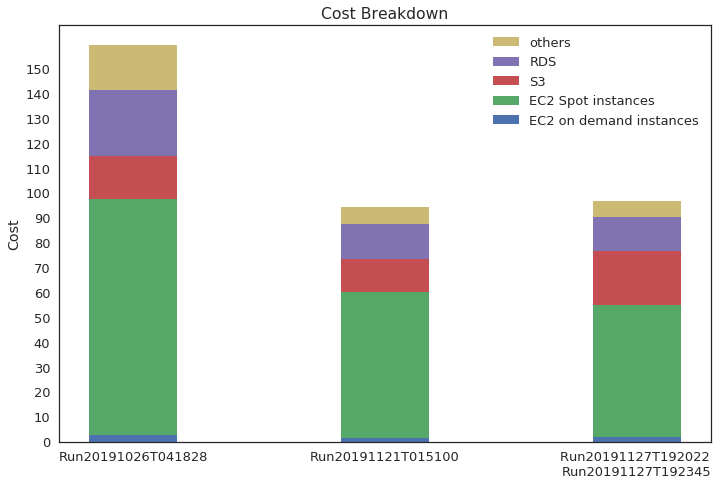
\includegraphics[width=0.7\textwidth]{billBreakdown.png}
\caption{Cost breakdown for each run}
\end{figure}


\subsection{Cost comparision and projection}

The raw input exposures in the HSC-RC2 tract=9615 workflow contains $\sim$0.2TB from 112 visits.
Only the CCD images overlapping the tract area were included in the workflow; so only $\sim$122 GB of raw inputs are used.
Compared to one night of LSST data in full operations, this is only $\sim$11\% in the number of visits, or $\sim$2\% in the data volume.
In our test runs, one tract of the DRP test workflow cost around \$95.

The same tract of data were processed on the NCSA Verification Cluster using Generation 2 Science Pipelines from the same \texttt{w\_2019\_38} release (\jira{DM-21386}).
The equivalent workflow, including single frame, coadd, and multiband processing, took 17.8 node-hours.
The cost of the current NCSA Verification Cluster (not including labor) is $\sim$\$0.017 per core-hour, or $\sim$\$0.408 per node-hour (\citeds{DMTN-135}).
Therefore we may think that the Generation 2 version of the same processing cost \$7.26.
This execution time was shorter than the average tract exeuction time, 59 node-hours per HSC-WIDE tract, in the S18 HSC-PDR1 reprocessing (\url{https://confluence.lsstcorp.org/display/DM/S18+HSC+PDR1+reprocessing}).
But that run was based on a release from 2018, and the performance is known to vary.
\url{https://confluence.lsstcorp.org/display/~sthrush/Node+Utilization+for++HSC-RC2+Reprocessing+Jobs} provides an example how execution time of HSC-RC2 changed between different versions of the LSST Stack in 2018.
The performance differences between Generation 2 and Generation 3 Science Pipelines is not well understood either.

Another data point is the same HSC-RC2 tract=9615 workflow processed on the NCSA Verification Cluster and Oracle database using Generation 3 Science Pipelines from the \texttt{w\_2019\_28} release (\jira{DM-19915}).
It took 8.8 hours on 10 nodes of the NCSA Verification Cluster; the nominal cost was then $\sim$\$36.
We note that the cumulative job wall time was 36.3 days in the \texttt{w\_2019\_28} run, much shorter than our run on AWS with \texttt{w\_2019\_38} where the cumulative job wall time was around 62 days (Table \ref{tab:runSummary}).
In the newer LSST Stack versions there are more jobs in total for this workflow.
But we do not know if the difference is dominated by the LSST Stack versions, infrastucture, or other factors.

Following \citeds{DMTN-135} we scale the cost with the input data size.
To estimate cost we multiply the nominal cost per input data by the estimated size of LSST data.
In one of our tests, we doubled the input size to explore how it scales up.
It scaled roughly linearly in cost and total compute resources.
In wallclock time, it did not take longer because more EC2 instances could be deployed.
For LSST DRP, there will be annually 1911 TB of raw science data with lossless compression.
Based on an input size of 122 GB and a cost of \$95 from our DRP test workflow, if the scaling relationship holds, the LSST processing would cost $\sim$\$1.5 million for the first year of DRP.
Note that this is a very crude estimate from a simple scaling.
Also, there are many ways to improve the efficiency and the \poc~project did not put effort into cost optimization.
AWS has pre-purchase plans and other discounts that may help further reducing the cost.


\section{Potential Improvements and more lessons learned} \label{sec:future}

In this session we describe issues we have encountered during the execution and ideas on how to improve the code or the instance and workflow management.
We discuss both intermittent failures that we understand and expect to occasionally encounter even in production, as well as higher level design or tooling improvements.

\subsection{Intermittent failures}

Failures can occur due to non-pipeline issues such as underlying infrastructure.
The fault rate may be small but as we scale up we start to encounter some.
Some examples are listed below; most seem transient.


\begin{enumerate}
\item Database connection timeout.
Attempting to connect to the RDS instance failed.
\begin{lstlisting}[style=basherror]
sqlalchemy.exc.OperationalError: (psycopg2.OperationalError) could not connect to server: Connection timed out
\end{lstlisting}
\item
After a file was added to a S3 bucket and during ingestion in the Butler registry, S3 reported a file does not exist.
This will be fixed in \jira{DM-22201}.
\begin{lstlisting}[style=basherror]
FileNotFoundError: File at 's3://hsc-rc2-test1-hfc/repo-w38/hfc30/srcMatchFull/1316/srcMatchFull_1316_24_HSC_17.fits' does not exist; note that paths to ingest are assumed to be relative to self.root unless they are absolute.
\end{lstlisting}
\item S3 read timeout before science processing started in a job.
\begin{lstlisting}[style=basherror]
botocore.exceptions.ReadTimeoutError: Read timeout on endpoint URL: "None"
\end{lstlisting}
\item Worker out-of-memory while running jobs.
For the same pipeline and input data, this is reproducible.
But we may not always have accurate memory usage prediction for any input data before running the jobs.
We can configure HTCondor to increase the memory requirement in the retry.
However sometimes OOM crashed the instances and appeared as a network issue which is not  desirable behaviour.
\item Launching HTCondor Annex workers failed with connectivity check collector issues.
\begin{lstlisting}[style=basherror]
Connectivity check found wrong collector (f5fc15573ffb9c93 vs a006066e73c412da).
\end{lstlisting}
\item Dataset ConflictingDefinitionError.
In rare occassions we observed dataset conflict errors from the registry without obvious reasons such as duplicate collection names or retries.
\jira{DM-21201} has refactored the code to robustify such transactions.
It could also be related to Spot instances getting terminated;
see next section on failure recovery.
\item Database instance not sized big enough.
We have seen
\begin{lstlisting}[style=basherror]
psycopg2.OperationalError: out of shared memory
\end{lstlisting}
and
\begin{lstlisting}[style=basherror]
sqlalchemy.exc.OperationalError: (psycopg2.OperationalError) FATAL:  remaining connection slots are reserved for non-replication superuser connections
\end{lstlisting}
These were resolved by increasing \texttt{max\_locks\_per\_transaction}, the cache size, and \texttt{max\_connections}.
\end{enumerate}


\subsection{Alternative architecture designs}

%In this \poc, we discussed different architecture designs but did not pursue all of them due to time constraints.

One prominent idea was to use HTCondor utilities to transfer files from and to S3, rather than relying on the Data Butler to communicate directly with S3.
In this design HTCondor controls all file transfers, and all datasets are declared in the execution workflow.
This design is enabled by a data transfer plug-in that was recently added to HTCondor.
In each job there would be a local POSIX data repository for all data access.
Utilities would be needed for determining, based on the Quantum Graph, the URLs of datasets that need to be transferred; for setting up the local Butler registry; and for ingesting the HTCondor-transferred S3 datasets into the main Butler registry.
This additional work was not able to be scheduled as part of the PoC.
A benefit of this approach is the potential for optimizing bulk data transfers.

With respect to the database, we discussed the possibility of each job having its own fast local SQLite registry.

After each job finishes, registries are then collated into the central database.
This is a subset of the previous design alternative, with only the registry being localized and not the datasets.
Besides simplifying failure recovery, another benefit is to avoid potential bottlenecks related to large scale parallel SQL transactions by bundling multiple transactions together and handling database connections in a centralized manner.
This envisions a fully shared-nothing architecture, but implementing this requires more thorough design work in conjunction with the Generation 3 Middleware development.
Current dependance on conflict-resolution of registry inserts is potentially a complete blocker to this approach.


\subsection{Tooling improvements}

More generally, improvements in and tooling rise to prominence.
We discuss some ideas below.

\begin{enumerate}
\item \textbf{Better job failure recovery strategies}.
Our jobs write directly to the S3 bucket and the RDS instance via the Data Butler.
If a job fails in a state that partial outputs are written but the job does not fully finish, recovery is not trivial.
Such failed partial writes are handled on the registry side the DBMS but on the datastore side they are handled by wrapping failable transactions in a transaction context manager.
The context manager takes a callable that then proceedes with the cleanup.
For S3 datastore, at the time of writing, the utility functions preforming the cleanup have not yet been written (in progress).
The larger issue with job failures is the lack of DRP workflow failure handling.
There is no way yet to reliably pause the DAG execution, overwrite files from a failed job, or other ways to handle such scenarios.
\item \textbf{Container based software stack}.
We have found it tricky to handle the LSST stack installation, dependencies, and environments to be used together with other software.
One possible way to avoid the headaches is to use docker based stack releases.
This may also ensure consistency of software on the master and the workers more easily, as well as improve shareability.
\item \textbf{Better cluster management tooling}.
Our current operational approach requires manually deploy suitable types and sizes of fleets based on our understanding of the overall workload.
Strategies on the instance choices and timing of requests therefore affect the cost, and manual adjustments are usually needed to reduce cost.
Annex can remove idle instances out of the condor pool but may not terminate the instances until the lease expires.
Also once instances drop out of the pool they can't be added back easily.
Tooling become essential for the operations.
For example we may use scripts to auto-scale the Annex condor pool based on the current demand for resources, or based on predictng resource demands from the Quantum Graph.
The execution overheads from idle instances may be mitigated by utilizing some of other AWS services, such as \href{https://aws.amazon.com/swf/}{Simple Workflow service (SWF)} or \href{https://aws.amazon.com/batch/}{AWS Batch} service.
This may bind the solutions strictly to AWS, a disadvantage of such adoption.
\item \textbf{End-to-end CI}.
This should include all operational components to do an end-to-end run.
This includes Butler repo generation, registry generation, Quantum Graph generation, job composition, workflow translation, job execution, and so on.
Many of the components were in the development phase and workarounds were used during the PoC.
For example a native Generation 3 ingestion was not available so a Gen2-to-Gen3 conversion was needed, and in fact many of the registries were migrated to RDS partially manually by executing bespoke scripts made specifically for such purpose that are not generally portable cross backwards-incompatible changes to the Middleware code.
As we put together the pieces, the absence of to do so in an automatic fashion became a key burden.
In retrospect we probably should have invested more time to automate the end-to-end workflow, even with workarounds, but the efforts were plagued by the lack of a canonical ingest tool.
Additionally, the DM team has concerns in the long execution time from overly-inclusive CI tests.
Adding S3 datastore CI tests to the default CI suite would double the total CI execution time.
\item \textbf{Credential handling}.
Security concerns received special attention in the \poc.
Natively none of the Middleware code requires the credentials to exist on the instance in plain text, even though they support that option.
Authentication can be performed via \href{https://docs.aws.amazon.com/IAM/latest/UserGuide/id_roles.html}{Identity and Access Management Roles} to both S3 and RDS services.
IAM Role authentication is more secure than other authentication methods, but require understanding of how AWS security and permissions work and sometimes require tedious setup.
For example for RDS IAM access an account admin needs to create the IAM Role then DB admin needs to log in to the DB interactively and create a role with rds\_iam permissions and then also grant usage priviledges on the DB schema, tables etc.
While we have tried an IAM setup in the \poc~we often stored credentials onto the master and worker instances in \texttt{\~{}/.lsst/db-auth.yaml}, \texttt{\~{}/.aws/credentials} or in environmental variables which is not the best practice of handling the access.
Utilities and tooling that help speed up such setup would be highly desireable.

\item \textbf{Robustify and give better error messages}.
It has been observed that sometimes the error messages could be misleading.
Also, scaling tests of a more substantial size are critial to find breaking points and bottlenecks.
\item \textbf{Other AWS services}.
Services such as \href{https://aws.amazon.com/batch/}{AWS Batch} and \href{https://aws.amazon.com/glue/}{AWS Glue} could potentially offer powerful tools to our use cases.
AWS Batch provides EC2 lifecycle management and workflow control, which may reduce the cost of our EC2 usage.
AWS Glue provides extract, transform, and load (ETL) services with respect to our S3 storage usage, which may improve our data warehousing experience and form Data Lake.

\end{enumerate}

\section{Summary}

In this \poc~project we have demonstrated the feasibility of LSST DRP data processing on the cloud.
We implemented AWS backends in the LSST Generation 3 Middleware, allowing processing entirely on the AWS platform using AWS S3 object store, PostgreSQL database, and HTCondor software.
We analyzed cost usage in our test execution, and estimated cost for larger processing campaigns.
We showcased our progress in a live demonstration in the LSST Project Community Workshop in Aug 2019, as well as a \href{https://confluence.lsstcorp.org/display/DM/Tutorials+at+the+Kavli+workshop}{hands-on tutorial in the Petabytes to Science Workshop} in Nov 2019.
Ideas of improvements necessary for larger-scale production are identified and discussed.


\appendix
% Remove this when you strart your paper
%\section{Appendix: implementing new features in Data Butler}
\label{sec:butler}

A major focus of the \poc~was to implement, and investigate issues related to, an S3 backed Datastore and a PostgreSQL backed Registry.
This appdendix describes the implementation process.

At the time the \poc~project began, Generation 3 Data Butler implemented \texttt{PosixDatastore}, a local or shared filesystem datastore, and a SqliteRegistry.
OracleRegistry followed soon after the \poc~work began.
Initially the focus was on implementing an S3 backed datastore called S3Datastore.
The interface between AWS services and LSST Stack would be based on the official AWS SDK called boto3.
In March 2019, Dino Bektesevic visited Tim Jenness for this work and implemented the early versions of a new module in the \texttt{daf\_butler} called \texttt{s3utils}, an \texttt{S3Datastore} class, the \texttt{PosixDatastore} equivalent, and a set of appropriate unit tests that demonstrated its functionality and correctness.
The unit tests for the datastore utilize the \texttt{moto} library which mocks requests and responses sent to AWS services, so that no additional external infrastructure is required to use it.
\texttt{PostgreSqlRegistry} class was implemented partially during the visit and completed shortly after the visit.
The initial implementation showcasing the required changes to the code was submitted as a Draft Pull Request \href{https://github.com/lsst/daf_butler/pull/147}{PR-147} in \texttt{daf\_butler}.

The tentative implementation revealed issues with how the Data Butler treated Uniform Resource Identifiers, or URIs, which were, at the time, not being handled correctly, as per standards defined in \href{https://tools.ietf.org/html/rfc3986}{FC-3986}, by the \texttt{Location} class.
In May 2019 \jira{DM-19916} resolved the issues with the \texttt{ButlerURI} class.
Major efforts were then invested into refining the newly added code to the level of production quality as well as updating the remaining Generation 3 Butler to use the updated \texttt{ButlerURI} code instead.
Every call to OS functionality had to be generalized to take a URI and from it determine the appropriate operation - a call to OS functionality, a AWS operation or something else.
This led changes in \texttt{Butler}, \texttt{Config}, \texttt{ButlerConfig} and YAML Loader classes.
These changes made the design of Data Butler more general and readily extesible to alternative cloud providers.

Further integration of the S3 backend required a change to Formatter classes to enable data serialization and deserialization to and from bytes.
Formatters present interfaces for reading and writing of Python objects to and from files.
They are the mechanism underlying how Data Butler is capable of presenting data as science products in the form of Python objects, abstracting away the underlying file types.
Modifications were made to \texttt{JsonFormatter}, \texttt{PickeFormatter}, \texttt{YamlFormatter}, \texttt{PexConfigFormatter} and the generic abstract class \texttt{Formatter}.
This concluded the last of changes required for \texttt{S3Datastore} integration and the code was merged in \href{https://github.com/lsst/daf_butler/pull/179}{PR-179} in \texttt{daf\_butler} (\jira{DM-13361}).
It became apparent that similarities were shared between \texttt{PosixDatastore} and \texttt{S3Datastore}, and would be shared by other future datastore implentations.
This prompted \jira{DM-21009} to reduce code duplication in the general datastore code.

\texttt{PostgreSqlRegistry} was added afterwards.
The initial implementation from March 2019 was based on \texttt{OracleRegistry}.
Similarities between the two implementations led to a re-implementation of the generic \texttt{SqlRegistry} class in July.
Problems were caused, for both Oracle and PostgreSQL, by the table naming conventions and additionally, for PostgreSQL, the table views did not conform to the assumptions made.
In July the \texttt{PostgreSqlRegistry} was re-implemented in terms of the more general \texttt{SqlRegistry} and a new SQLAlchemy expressions compiler was written, so that table views could be generated correctly.
The policy for additional registry implementations was not to accept associated unit tests, as they are dependent on existing outside architecture, meant that checking whether it worked or not had to be based on manually executing actual data workflows.
In July and Auguest Dino Bektesevic migrated existing SQLite registries to PostgreSQL and with Hsin-Fang Chiang started testing using the ci\_hsc workflow on AWS.
The code was merged into the master branch of \texttt{daf\_butler} in August with \href{https://github.com/lsst/daf_butler/pull/161}{PR-161}.
A major issue was then discovered when issuing rollback statements during error recovery stemming from assumptions made when implementing how all of the current SQL registries handle errors during transactions.
A stopgap solution, that works for all currently implemented registries, was implemented in \jira{DM-21210} and a more complete solution was implemented later in \jira{DM-21201}.

Security and authorization issues were handled for both \texttt{S3Datastore} and \texttt{PostgreSqlRegisty}.
Significant attention was paid to preserving the flexibility of the authentication in order to be able to incorporate external authenticators such as Oracle Wallets and AWS IAM Roles and Policies.
There were several different iterations and improvements made to the authentication implementation (\jira{DM-20992}, \jira{DM-21146}, \jira{DM-21222}) that resulted with the current implementation.
\jira{DM-20992} re-implemented the \texttt{DbAuth} module that was previously C++ wrapped in the Generation 2 Butler \texttt{daf\_persistence} to pure Python in the Generation 3 Butler, so that the module would support basic file based authentication in absence of external authentication methods.
Additional layers of security were achieved through EC2/S3/RDS interfaces by IP white/blacklisting , IAM, Policies etc.
These policies can be very granular, affecting individually selected objects, Bucket-wide to placing all instances on the same, externally innaccessible, Virtual Private Network (VPN).

Adding the support for AWS into the Data Butler exercised a significant fraction of the Generation 3 Data Butler codebase.
During the process many faults and undesired behaviors were discovered and solved.
Issues encountered challenged the Data Butler implementation, as well as assumptions made during the implementation.
Recounting the wide list of major improvements to the codebase, hopefully, reveals how productive this exercise has been in helping generalizing and strengthening the whole Generation 3 Data Butler codebase.

\section{Appendix: PostgreSQL performance}

Versions of the Generation 3 Middleware prior to and including w\_2019\_38 did not attempt to optimize database performance.
In those versions, the QuantumGraph was created by issuing a very large SQL statement that, effectively, created a cartesian product between many of the tables in the registry.
The results of this large query were then parsed in Python, and a slew of many different, small, follow-up queries were issued.
The Generation 3 Middleware team reported that on average it took 0.5 to 1.5h to create QuantumGraphs for tract-size DRP workflows with Oracle on NCSA infrastructure using these versions.
In our tests we were unable to create even the simplest QuantumGraphs, even after doubling the RDS instance resources, and were forced to abort multiple times after 30+h of execution.
None of the performance metrics available showed heavy hardware loads.


An issue seemed to be that all the views materialized completely on disk.
Even when the views were part of larger statements, in which the outer statements had strict constraints on them, the outer constraints did not seem to penetrate to the view statement.
This behavior caused the severe performance problem.
Below is an abbreviated query plan for the simplest case of \lstinline[basicstyle=\ttfamily]{select * from visit_detector_patch_join limit 4;} that suffered from the described issue.

\begin{lstlisting}[style=sqlprompt]
Limit ....
(actual time=12732.766..12732.774 rows=4 loops=1)
->Unique ....
(actual time=12732.765..12732.770 rows=4 loops=1)
  ->Sort ....
(actual time=12732.764..12732.767 rows=6 loops=1)
    Sort Key: ....
    Sort Method: external merge  Disk: 209008kB
    ->Hash Join ....
(actual time=763.846..1524.504 rows=4642107 loops=1)
      Hash Cond: ....
      ->Seq Scan on ....
(actual time=0.008..16.289 rows=206960 loops=1)
      ->Hash ....
(actual time=763.723..763.724 rows=3259107 loops=1)
        Buckets: 65536  Batches: 64  Memory Usage: 3635kB
        ->  Seq Scan on patch_skypix_join ....
(actual time=0.006..240.128 rows=3259107 loops=1)
Planning time: 0.323 ms
Execution time: 12759.391 ms
\end{lstlisting}

Note that the total materialized size of the view on disk was 200MB and that it took 12 seconds to retrieve only 4 results!
We were unable to find a way to disable the view materialization in PostgreSQL without changing the SQL queries generated by the middleware.

One solution we found was to manually redefine the views as materialized views instead, adding triggers that recreate the views on any insert statement to the underlying tables that make the view, and then adding indexing onto the materialized views.
This reduced the time of the QuantumGraph creation to be comparable to that reported by the Generation 3 Middleware team using Oracle.
The query plan for the same SQL select statement as described above now looks like:

\begin{lstlisting}[style=sqlprompt]
Limit ....
(actual time=0.009..0.010 rows=4 loops=1)
->Seq Scan on visit_detector_patch_join ....
(actual time=0.008..0.008 rows=4 loops=1)
Planning time: 0.053 ms
Execution time: 0.021 ms
\end{lstlisting}

Recently \jira{DM-17023} reworked and completely re-implemented the SQL schema and data model for the registries.
We have not yet tested the performance of the new registry schema in PostgreSQL.
Because all SQL statements are generated dynamically, guaranteeing execution plan stability and performance is difficult.
Our execution tests used a particular version of the LSST Software Stack and we optimized a specific set of queries.
The optimization strategy might not apply to new versions of the software.
Furthermore, the behaviors may differ between different database management systems (DBMSs).
Testing in one DBMS does not guarantee the performance for others.

% Include all the relevant bib files.
% https://lsst-texmf.lsst.io/lsstdoc.html#bibliographies
\section{References} \label{sec:bib}
\bibliography{local,lsst,lsst-dm,refs_ads,refs,books}

% Make sure lsst-texmf/bin/generateAcronyms.py is in your path
\section{Acronyms} \label{sec:acronyms}
%\input{acronyms.tex}

\end{document}
